%%%%%%%%%%%%%%%%%%%%%%%%%%%%%%%%%%%%%%%%%%%%%%%%%%%%%%%%%%%%%%%%%%%%%%%%%%%%%%%%%%
\begin{frame}[fragile]\frametitle{}
\begin{center}
{\Large Introduction to Yog Shastra}
\end{center}
\end{frame}

%%%%%%%%%%%%%%%%%%%%%%%%%%%%%%%%%%%%%%%%%%%%%%%%%%%%%%%%%%%
\begin{frame}[fragile]\frametitle{Yog (योग) == Asana (आसन)?}
When people hear the word ``Yoga''

	\begin{itemize}
	\item You imagine someone doing contorted, nearly impossible postures.
	\item Or some skeleton siting aloof with long hair, beard
	\item Or anyone earing full saffron robe
	\end{itemize}

\end{frame}

%%%%%%%%%%%%%%%%%%%%%%%%%%%%%%%%%%%%%%%%%%%%%%%%%%%%%%%%%%%
\begin{frame}[fragile]\frametitle{Yog (योग) == Asana (आसन)?}

	\begin{itemize}
	\item Well, these could be some, but rather less important aspects of Yog
	\item Yog (योग, not Yoga ie योगा) is more about mind than getting your leg behind the neck and still keeping the face straight!!
	\item ``Patanjali Yog Sutra (पतञ्जलि योग सूत्र)'' is the most concise, complete and authoritative work on Yog.
	\item Out of 195 sutras, only 3 discuss Yog postures or asanas (आसन)
	\item And he says, ``Sthir Sukham Asanam (स्थिर सुखम आसनम्)'', Postures should be steady and pleasant (2:46), a balance of efforts and ease.
	\end{itemize}

\end{frame}

%%%%%%%%%%%%%%%%%%%%%%%%%%%%%%%%%%%%%%%%%%%%%%%%%%%%%%%%%%%
\begin{frame}[fragile]\frametitle{Popularity}

Popularity of Yog is due to:
	\begin{itemize}
	\item Maintains wellness
	\item As a complementary approach to recover from illness
	\item To manage stress and trauma
	\end{itemize}

But, clearly understand that Yog is not a replacement medical procedures, especially the emergencies.

\end{frame}

%%%%%%%%%%%%%%%%%%%%%%%%%%%%%%%%%%%%%%%%%%%%%%%%%%%%%%%%%%%
\begin{frame}[fragile]\frametitle{International Yoga Day (IYD)}
21st June, every year. Why this day/date?

   \begin{columns}
    \begin{column}[t]{0.4\linewidth}
	
\begin{center}

\includegraphics[width=0.5\linewidth,keepaspectratio]{images/yog16}
\end{center}


    \end{column}
    \begin{column}[t]{0.6\linewidth}
		\begin{center}
		\textit{``By proclaiming 21 June as the International Day of Yoga, the General Assembly has recognized the holistic benefits of this timeless practice and its inherent compatibility with the principles and values of the United Nations.'' -    Ban Ki-moon (United Nations Secretary-General)}
	\end{center}

    \end{column}
  \end{columns}

\end{frame}


%%%%%%%%%%%%%%%%%%%%%%%%%%%%%%%%%%%%%%%%%%%%%%%%%%%%%%%%%%%
\begin{frame}[fragile]\frametitle{IYD Celebrations 2015}
The first IYD \ldots

\begin{center}
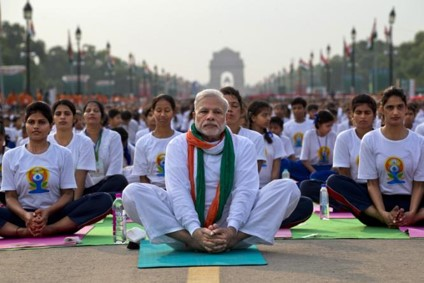
\includegraphics[width=0.8\linewidth,keepaspectratio]{images/yog17}
\end{center}

\end{frame}


%%%%%%%%%%%%%%%%%%%%%%%%%%%%%%%%%%%%%%%%%%%%%%%%%%%%%%%%%%%
\begin{frame}[fragile]\frametitle{PUBMED Search June 21-2015}

Number of articles found and the search terms: 

	\begin{itemize}
	\item 3052 : Yoga Therapy
	\item 144 : Yoga back pain
	\item 102 : Yoga Low back Pain
	\item 32 : Yoga neck pain
	\item 565 : Yoga Stress
	\item 263 : Yoga Cancer
	\item 257 : Yoga cardiovascular
	\item 137 : Yoga Hypertension
	\end{itemize}

\tiny{(Ref: YOGA for Wellness: Gentle Yoga Practice - Maruti Ram Gudavalli )}


\end{frame}

%%%%%%%%%%%%%%%%%%%%%%%%%%%%%%%%%%%%%%%%%%%%%%%%%%%%%%%%%%%
\begin{frame}[fragile]\frametitle{Sample Article}

\begin{center}
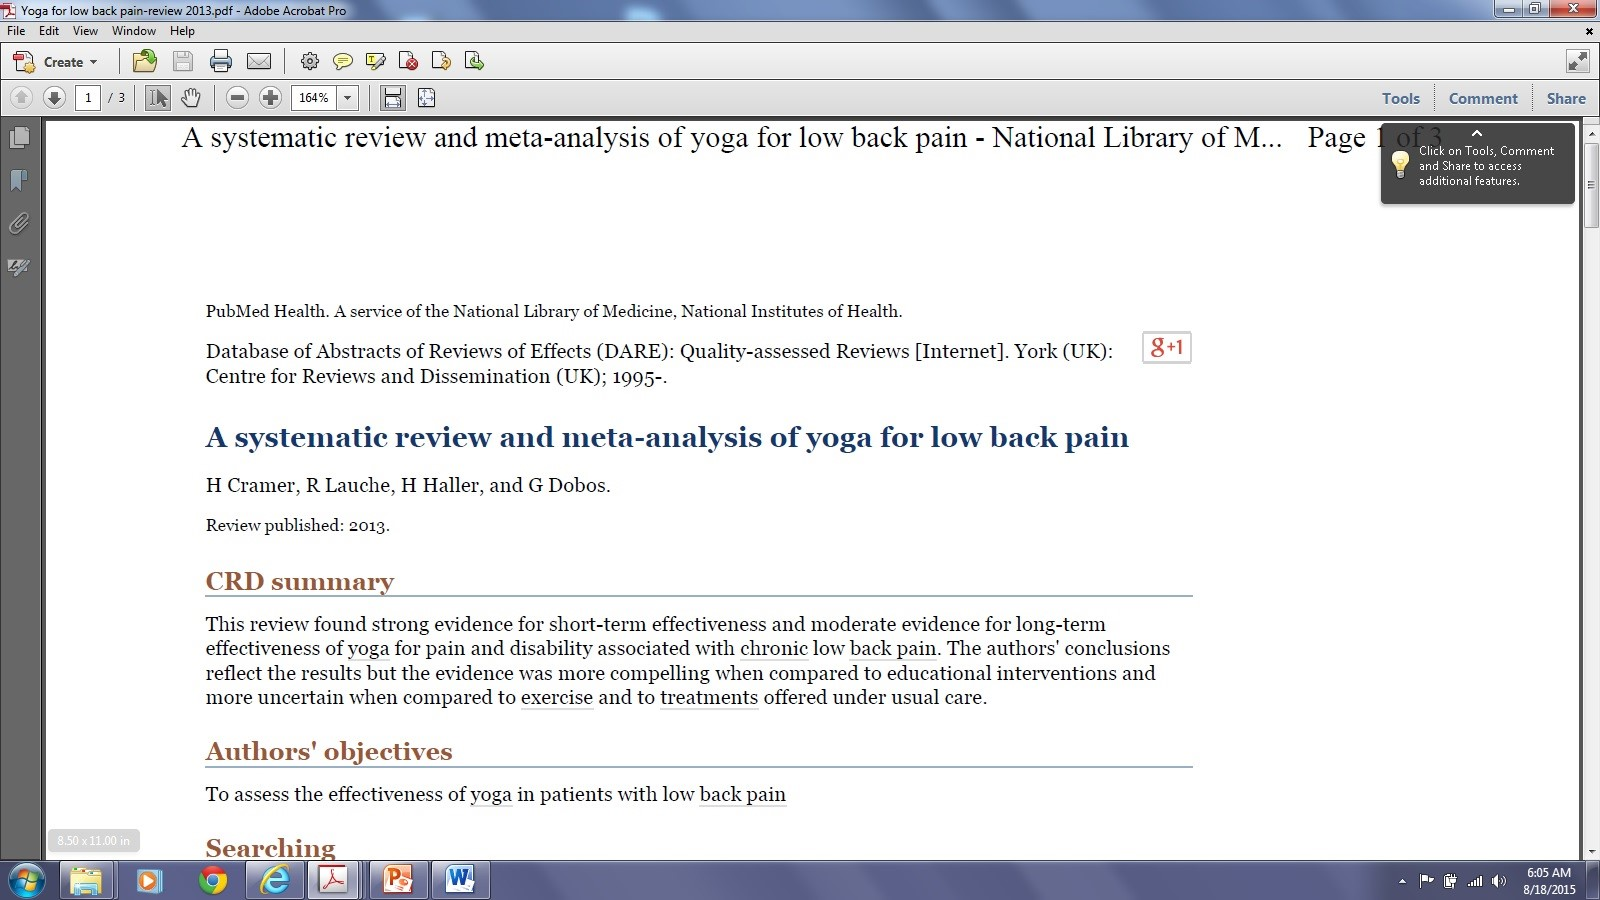
\includegraphics[width=0.8\linewidth,keepaspectratio]{images/yog18}
\end{center}

\tiny{(Ref: YOGA for Wellness: Gentle Yoga Practice - Maruti Ram Gudavalli )}


\end{frame}



%%%%%%%%%%%%%%%%%%%%%%%%%%%%%%%%%%%%%%%%%%%%%%%%%%%%%%%%%%%
\begin{frame}[fragile]\frametitle{What is Yog?}

Yog (योग) is derived from verb-root yuj (युज्) means to unite

Yog is a path that leads to union of:
	\begin{itemize}
	\item Physical body
	\item Mental body
	\item Psychological body
	\item Spiritual body
	\end{itemize}

\end{frame}

%%%%%%%%%%%%%%%%%%%%%%%%%%%%%%%%%%%%%%%%%%%%%%%%%%%%%%%%%%%
\begin{frame}[fragile]\frametitle{Ashtang Yog (अष्टांग योग)}
8 facets (ang, अङ्ग) of Yog:
	\begin{itemize}
	\item Yama यम : What not to do
	\item Niyama नियम : What to do on a regularly
	\item Asana आसन : Postures and exercises
	\item Pranayama प्राणायाम : Breathing Exercises
	\item Pratyahara प्रत्याहार : Controlling senses
	\item Dharana धारणा: Focus
	\item Dhyana ध्यान: Meditation
	\item Samadhi समाधि :  Realization

	\end{itemize}

\end{frame}

%%%%%%%%%%%%%%%%%%%%%%%%%%%%%%%%%%%%%%%%%%%%%%%%%%%%%%%%%%%
\begin{frame}[fragile]\frametitle{Definitions of Yog?}

	\begin{itemize}
	\item \textbf{Patanjali}: yogas-chitta-vrutti-norodhah (योगस्चित्तवृत्तिनिरोध:) (YogSutra 1:2): Yoga is the cessation of modifications of the mind
	\item \textbf{Yoga-Vasishta}: manah prashamanah upayah yog itibhidyate (मन: प्रशमन: उपाय: योग इत्याभियते) (Yog Vashishth 3:9:32): Yoga is a skillful way to calm down the mind
	\item \textbf{Bhagavad Gita}: yogah karmasu kaushalam (योग: कर्मसु कौशलम्:) (Bhagvad Gita 2:50): Yoga is dexterity in action
	\item \textbf{Bhagavad Gita}: samatvam yog uchyate (समत्वं योग उच्यते) (Bhagvad Gita ?:??): Equanimity towards everything is Yog.	
	\end{itemize}

\end{frame}

%%%%%%%%%%%%%%%%%%%%%%%%%%%%%%%%%%%%%%%%%%%%%%%%%%%%%%%%%%%
\begin{frame}[fragile]\frametitle{Contradictions in Definitions of Yog}

	\begin{itemize}
	\item There were two systems of Yog. One had gotten lost. Krishna is trying to revive the lost one, in Gita श्रीमद्भगवद्गीता. This goes for DOING ACTION
	\item The more known one is the Patanjali Yog. This goes for STOPPING ACTION.
	\item Patanjali type of Yog is mentioned in Upanishads also. Go to secluded place, in the forest, in the cave, by the stream, etc. (Ref: Mokshadhrama मोक्षधर्म)
	\item Even Arjun अर्जुन had this understanding. He gets confused. Why do the action/battle?
	\item Krishna does not reject renunciation type of yoga, but keeps it aside (Raj राजयोग / dhyan ध्यानयोग in gita itself) and says its not for you (Arjun), you need Action Yoga. (karma कर्मयोग)
	\item Karma becomes yoga when only you have no attachment to it. Doing the ACTION as an offering to the Lord (Krishna कृष्ण)
	\item Even Patanjali Yog is a practice. Its Asana आसन aspect is fully action oriented. But thats just to prepare you for the final goal of Samadhi (समाधि)
	\end{itemize}

\tiny{(Ref: Edwin Bryant sutras - Kristen Vrabel)}


\end{frame}


%%%%%%%%%%%%%%%%%%%%%%%%%%%%%%%%%%%%%%%%%%%%%%%%%%%%%%%%%%%
\begin{frame}[fragile]\frametitle{Why Yog?}

	\begin{itemize}
	\item State of cessation of misery is called as moksh (मोक्ष), kaivalya (कैवल्य), nishreyas (निश्रेयस), parampad (परमपद).
	\item One can attain this state only when we have clear understanding (sukshma gyan सुक्ष्म ज्ञान) of world around.
	\item For this understanding, one needs specific state of mind (chitta vishuddhi चित्त विशुद्धि)
	\item To attain this state of mind, sages have advised many ways, and one of the ways is Yog (Yog dasrhan योगदर्शन)
	\item Yogsharta by Patanjali has given ways of yog darshan to attain moksh.
	\end{itemize}

\tiny{(Ref: पातंजल योग सूत्र | Yog Darshan - Yoga And Ayurveda Science Youtube channel)}

\end{frame}

%%%%%%%%%%%%%%%%%%%%%%%%%%%%%%%%%%%%%%%%%%%%%%%%%%%%%%%%%%%
\begin{frame}[fragile]\frametitle{ योग दर्शन Yog Darshan}

	\begin{itemize}
	\item Removal of human sufferings through practice of yoga
	\item Explains purpose of life, reincarnation
	\item Experience of ultimate reality - self realization (kaivayla कैवल्य )
	\end{itemize}

\tiny{(Ref: Patanjali Yoga Sutra Dr Mrudula Chaudhari)}

\end{frame}

%%%%%%%%%%%%%%%%%%%%%%%%%%%%%%%%%%%%%%%%%%%%%%%%%%%%%%%%%%%
\begin{frame}[fragile]\frametitle{Canvas of Hindu Scriptures}

\begin{center}
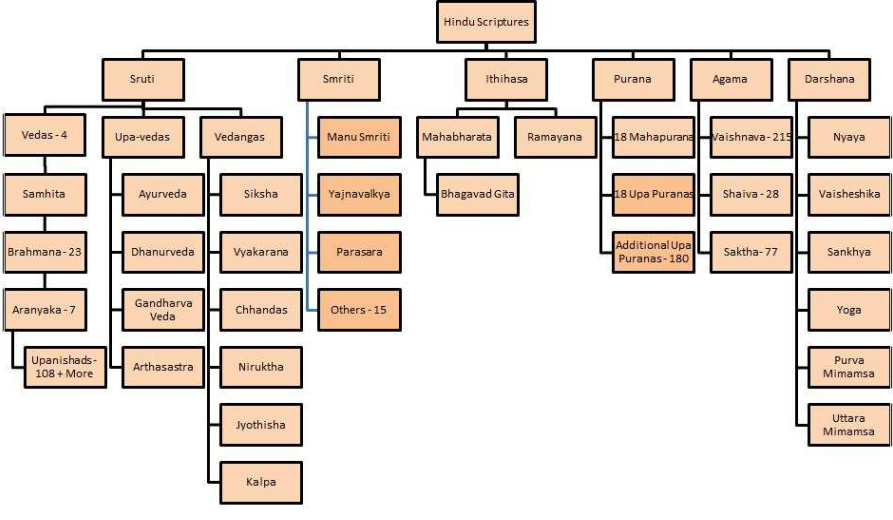
\includegraphics[width=\linewidth,keepaspectratio]{yog36}

\end{center}

  
  \tiny{(Ref: Patanjali Yoga Darshan- For AYUSH YOGA EXAM- Deepak D.Khaire)}

\end{frame}

%%%%%%%%%%%%%%%%%%%%%%%%%%%%%%%%%%%%%%%%%%%%%%%%%%%%%%%%%%%
\begin{frame}[fragile]\frametitle{दर्शन Darshan}

6 आस्तिक दर्शन (वेद प्रमाणं)
	\begin{itemize}
	\item Nyaya न्याय: Rishi Gautama ऋषि गौतम: Logical quest for god, phases of creation.
	\item Vaisheshika वैशेषिक: Rishi Kanada ऋषि कणाद: Science of Logic, futility of Maya माया.
	\item Sankhya साङ्ख्य: Rishi Kapil ऋषि कपिल: Eliminate Physical and mental pains and receive liberation.
	\item Yog योग: Rishi Patanjali ऋषि पतञ्जलि : Practice of meditation and postures for renunciation.
	\item Mimansa मिमान्सा: Rishi Jaimini ऋषि जैमिनी : Explains vedas are eternal and divine.
	\item Vedanta वेदान्त : Rishi Ved Vyas ऋषि वेद व्यास: Explains the divine nature of soul, Maya and creation.	
	\end{itemize}

३ नास्तिक दर्शन (वेद अप्रमाणं)

	\begin{itemize}
	\item Charvak न्याय
	\item Bauddha बौद्ध
	\item Jain जैन

	\end{itemize}
  \tiny{(Ref: Patanjali Yoga Darshan- For AYUSH YOGA EXAM- Deepak D.Khaire)}

\end{frame}
	

%%%%%%%%%%%%%%%%%%%%%%%%%%%%%%%%%%%%%%%%%%%%%%%%%%%%%%%%%%%%%%%%%%%%%%%%%%%%%%%%%%
\begin{frame}[fragile]\frametitle{}
\begin{center}
{\Large Basic Terms}
\end{center}
\end{frame}

%%%%%%%%%%%%%%%%%%%%%%%%%%%%%%%%%%%%%%%%%%%%%%%%%%%%%%%%%%%
\begin{frame}[fragile]\frametitle{ धर्म Dharma}

	\begin{itemize}
	\item Duties to be performed by everyone for a larger good
	\item Social order divinely sustained.
	\item Every person has a part to play, and each part is held to be necessary in some way to the ultimate end

	\end{itemize}

\tiny{(Ref: Philosophy III - The Yoga SPace - Chandrika Gibson)}

\end{frame}

%%%%%%%%%%%%%%%%%%%%%%%%%%%%%%%%%%%%%%%%%%%%%%%%%%%%%%%%%%%
\begin{frame}[fragile]\frametitle{ मोक्ष Moksh}

	\begin{itemize}
	\item One's eternal destiny, a release from all limitations \& restrictions
	\end{itemize}

\tiny{(Ref: Philosophy III - The Yoga SPace - Chandrika Gibson)}

\end{frame}

%%%%%%%%%%%%%%%%%%%%%%%%%%%%%%%%%%%%%%%%%%%%%%%%%%%%%%%%%%%
\begin{frame}[fragile]\frametitle{Guna गुण, प्रकृति}

	\begin{itemize}
	\item Sattva सत्त्व : उत्तम प्रकृति: Balance, Positive, Peace
	\item Rajas राजस: मध्यम प्रकृति: Activity, Energy, Excitement
	\item Tamas तामस: अधम प्रकृति: Inactivity, Negative, Apathy

	\end{itemize}

  
  \tiny{(Ref: Patanjali Yoga Darshan- For AYUSH YOGA EXAM- Deepak D.Khaire)}

\end{frame}

%%%%%%%%%%%%%%%%%%%%%%%%%%%%%%%%%%%%%%%%%%%%%%%%%%%%%%%%%%%
\begin{frame}[fragile]\frametitle{Mind मन}

	\begin{itemize}
	\item चित्त: stores input got from senses इंद्रिय into memory स्मृती
	\item अहङ्कार: decide what one likes, dislikes
	\item बुद्धि: decides true state of objects or events नीर क्षीर विवेक 
	\item मन: estimates good/bad-ness of the future events
	\end{itemize}

  
  \tiny{(Ref: mana sajjana मना सज्जना- Bhishmaraj Bam)}

\end{frame}